\documentclass[parskip=full]{scrartcl}
\usepackage{pdfpages}
\usepackage[utf8]{inputenc}
\usepackage[T1]{fontenc}
\usepackage[german]{babel}
\usepackage{hyperref}
\hypersetup{
	pdftitle={Pflichtenheft},
	bookmarks=true,
}
\usepackage{csquotes}

\usepackage{fancyhdr}%<-------------to control headers and footers
\usepackage[a4paper,margin=1in,footskip=.25in]{geometry}
\fancyhf{}
\fancyfoot[C]{\thepage} %<----to get page number below text
\pagestyle{fancy} %<-------the page style itself

\usepackage{xcolor}
\usepackage{framed}
\definecolor{shadecolor}{RGB}{220,220,220}
\usepackage{float}


\title{Android GO! App - Pflichtenheft}
\author{Gruppe 3}
\date{11.06.17}

% define custom lists
\usepackage{enumitem}
\usepackage{lipsum}

% add glossary
\usepackage{glossaries}
\makeglossaries
\newglossaryentry{System}
{
	name={System},
	description={Die Kombination aus Mobile App und Server},
}

\newglossaryentry{GO} %TODO anderen Namen finden
{
	name={GO},
	description={Ein Event in einer Gruppe, dem Mitglieder beitreten können, um ihren Standort mit anderen GO-Teilnehmern zu teilen},
	plural={GOs},
}
\newglossaryentry{Benutzer}
{
	name={Benutzer},
	description={Eine Person, die die App installiert und sich mit einem Benutzeraccount registriert hat bzw. plant dies zu tun},
}
\newglossaryentry{Anzeigename}
{
	name={Anzeigename},
	description={Ein im System nicht-eindeutiger Name, den der Benutzer jederzeit ändern kann},
}
\newglossaryentry{Hauptansicht}
{
	name={Hauptansicht},
	description={Ansicht, die geöffnet wird, sobald sich ein Benutzer angemeldet hat. Dies entspricht der Ansicht *GUI-Ansicht*},
}
\newglossaryentry{App}
{
	name={App},
	description={mobile Applikation, die auf dem Smartphone/Tablet des Benutzers installiert ist. Der Benutzer interagiert ausschließlich mit der Applikation und nicht mit dem Webserver direkt.},
}
\newglossaryentry{losgehen}
{
	name={losgehen},
	description={Die Änderung des Teilnahmestatus eines GOs von 'Bestätigt' auf 'Unterwegs'},
}

\def\threedigits#1{%
  \ifnum#1<100 0\fi
  \ifnum#1<10 0\fi
  \number#1}

\begin{document}

\begin{titlepage}
	\begin{center}
	%TODO evtl App-Logo ergänzen
	%\includegraphics[width=0.15\textwidth]{example-image-1x1}\par\vspace{1cm}
	{\scshape\LARGE \bfseries Pflichtenheft \par}
	\vspace{1cm}
	{\scshape\Large Praktikum der Softwareentwicklung \\ Sommersemester 2017\par}
	\vspace{1.5cm}
	{\huge\bfseries Android GO! App\par}
	\vspace{2cm}
	{\Large\itshape - Gruppe 3 -\par}
	\vfill
	{\bfseries erstellt von:\par}
	Arsenii Dunaev \\
	Florian Kröger \\
	Tina Maria Strößner \\
	Volodymyr Shpylka \\	
	\vfill
	% Bottom of the page
	{\large 11.06.17 \par}	
	\end{center}
\end{titlepage}

\tableofcontents

%TODO Gliederung ggfs nochmal überarbeiten
\newpage
\section{Zielbestimmung}
Die \gls{App} dient der Erleichterung und Strukturierung von Gruppentreffen. 
 Bei täglichen Vereinbarungen, ist die Kommunikation im Text-Format via WhatsApp und ähnlichen Apps unübersichtlich und unintuitiv. 
Dies wird durch die GO-App gelöst, indem wir Struktur in den Vereinbarungsprozess reinbringen.  
\subsection{Musskriterien}
% Anzahl Gruppen, Gruppenmitglieder, GOs, etc. beschränken
% grobe Zusammenfassung d. fktl. Kriterien (+ referenz auf die jeweiligen Funktionen)
% Aktualität der Standorte / Häufigkeit er Aktualisierung
% wann wird geclustert?

\begin{itemize}[itemsep=0pt]
	\item Benutzer  
	\begin{itemize}
	 	\item Registrierung
	 	\item Anmeldung
	 	\item Unterscheidung zwischen Administrator der Gruppe und ordentlichen Teilnehmer
	\end{itemize} 
	\item Gruppen
		\begin{itemize}
	 		%\item Jeder kann eine Gruppe erstellen und Nutzer in die Gruppe einladen
	 		%\item Jeder Teilnehmer der Gruppe kann ein Event in der Gruppe erstellen
	 		%\item Jeder Teilnehmer der Gruppe kann sich zum Event in der Gruppe anschließen
	 		%Das oben kommentiert sind eher schon Funktionalen Anforderungen
	 		\item Gruppen erstellen
	 		\item Events mit Eventdetails in der Gruppe erstellen 
	 		\item Zu den Gruppen eingeladen werden können
	 		\item Gemittelten Standort der Eventsteilnehmer anzeigen 
		\end{itemize}
\end{itemize}
	
\subsection{Wunschkriterien}
% Profilbilder
% Gruppenbilder
% Benachrichtigungen ??
\begin{itemize}
	\item Profilbilder
	\item Gruppenbild
	\item Benachrichtigungen (wie z.B. ''Event in 30 Minuten'', oder ''Jemand ist in der Nähe'')
\end{itemize}

\subsection{Abgrenzungskriterien}
% kein IM
% kein Social Media
% kein Live-Navigationssystem mit Routenplanungsfunkton, etc.
% Kontakte wrden nur innerhalb der Gruppen hinzugefügt
Diese App ist kein Instant Messaging Platform: Textnachrichten, Filesharing wie z.B. in WhatsApp werden nicht unterstützt.

\newpage
\section{Produkteinsatz}
\subsection{Anwendungsbereiche}
Die GO! App ist eine Software-Oberfläche, die speziell zur Organisation von Treffen (z. B. gemeinsames Essen im Café oder in der Mensa) entwickelt wird. Bei dem erfolgreichen gemeinsamen Losgehen wird der gemittelte GPS-Standort von Mitgliedern der Gruppe angezeigt.
 
\subsection{Zielgruppen}
Als Zielgruppe werden junge Leute und Erwachsene (13-50 Jahre alt) berücksichtigt, die sich regelmäßig mit Freunden verabreden und eine einfache App brauchen, um strukturierter ihre Treffen zu organisieren und ihre Freunde bei dem Losgehen zu finden.

\subsection{Betriebsbedingungen}\label{Betriebsbedingungen}
% mind. benötigte Android-Version -> 4.4
% funktionierende Netzwerkverbindung
% Zugriff auf GPS-Daten erlaubt
\begin{itemize}
	\item Die App braucht funktionierende Netzwerkverbindung auf dem Android Gerät.\\
	\item Der Zugriff auf GPS-Daten muss erlaubt sein.\\
	\item Die Benutzer müssen einen Google-Account besitzen, um sich in der App zu registrieren.
\end{itemize}

\newpage
\section{Produktumgebung}

\subsection{Software}
\begin{itemize}
	\item Client Seite:
	\begin{itemize}
		\item Android Version 4 (oder höher) wird auf dem Gerät verlangt.
	\end{itemize}
	
	\item Server Seite:
	\begin{itemize} 
        \item Apache Tomcat (Version 8).
		%\item MySQL-Datenbank. %TODO Brauchen wir eine Datenbank und wenn ja, welche benutzen wir dann?
    \end{itemize}
\end{itemize}


\subsection{Hardware}
% \subsection{Produktschnittstellen} --> inwiefern ist das im Pflichtenheft relevant?
\begin{itemize}
	\item Client Seite:
	\begin{itemize} 
		\item Internetfähiges Android Gerät. %(bei der Registrierung/Erstanmeldung eines neuen Gerätes wird ein Android-Gerät mit einer funktionierenden SIM-Karte verlangt).\\
	\end{itemize}
	
	\item Server Seite:
	\begin{itemize}
		\item Internetfähiger Server.
		\item Rechner, der die Ansprüche der o.g. Server-Software erfüllt.
	\end{itemize}		
\end{itemize}

\newpage

\section{Funktionale Anforderungen}
Im folgenden Abschnitt werden die funktionalen Anforderungen sowohl der Musskriterien, als auch der Wunschkriterien erläutert. Anforderungen, die die Wunschkriterien beschreiben (also nicht zwingend implementiert werden müssen) sind \colorbox{shadecolor}{farblich gekennzeichnet}.

\subsection{Benutzerkontofunktionen}

\subsubsection{Übersicht}
Die Benutzerkontofunktionen erlauben das Erstellen, Verwalten und Löschen von Benutzeraccounts im System.

\begin{figure}[H]
	\centering
	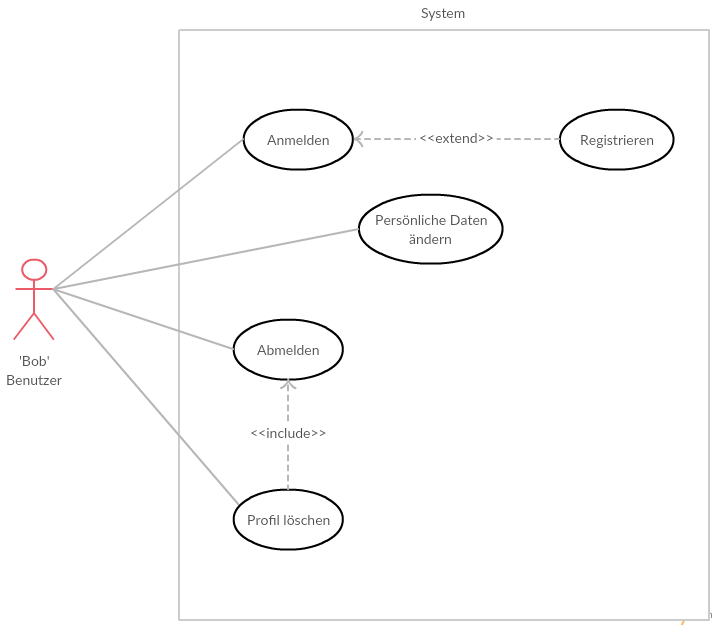
\includegraphics[width=.7\textwidth]{Use_Cases/use_case_Benutzerprofil.png}
	\caption{Use-Case Diagramm für Benutzerkontofunktionen}	
\end{figure}

\subsubsection{Funktionen}

\begin{enumerate}[label={\textbf{/F\protect\threedigits{\theenumi}0/}}, leftmargin=*]
	
	\item \textit{Registrieren}\label{Registrieren} \\ Ein beliebiger Benutzer, der zuvor die App auf seinem Andoid-Ger"at installiert hat und ein Google-Account besitzt, kann sich in der App registrieren un ein Benutzeraccount zu erstellen. Dazu muss der Benutzer sich auf dem Anmeldescreen (vgl. *GUI-Ansicht*) mit einem existierenden Google-Account anmelden (vgl. \ref{Anmelden}). Wird diese Funktion zum ersten Mal ausgeführt, wird vom System automatisch ein neuer Account für diesen Benutzer angelegt und der Benutzer in diesen Account eingeloggt. Bevor der Benutzer die App nutzen kann, muss er bestätigen, dass er mit einer eventuellen unanonymisierten Veröffentlichung seines Standortes einverstanden ist (vgl. \ref{Anonymisierung}). Wird dies nicht bestätigt, schlägt die Registrierung fehl.
	Bei erfolgreicher Registrierung kann sich der Benutzer ab sofort mit seinem Google-Account im System anmelden und Zugriff auf seinen Benutzeraccount erlangen.

	 	
	\item \textit{Anmelden} \label{Anmelden} \\ Ein Benutzer kann sich mithilfe seines Google-Accounts im System anmelden. Dazu ist sind folgende Eingaben des Benutzers erforderlich:
	\begin{itemize}
		\item E-Mail Adresse mit der der Benutzer bei Google registriert ist
		\item Passwort des Google-Accounts des Benutzers
	\end{itemize}
	Sind die Angaben korrekt wird der Benutzer vom System in sein GO-Benutzeraccount eingeloggt. Der Benutzer bleibt eingeloggt, bis er die Funktion \ref{Abmelden} ausführt, dies gilt auch für das zwischenzeitliche Schließen der App.
	
	%\item \textit{Benutzerkennung anfordern} \\ Ein Benutzer kann, sollte er sein Passwort vergessen haben, seine Benutzerkennung anfordern und eine neues Passwort setzen. Wird auf dem Anmeldescreen (vgl. *GUI-Ansicht*) die 'Passwort vergessen'-Option gewählt, schickt der Server dem Benutzer eine SMS mit einem Zugangscode. Dieser Zugangscode ist 10min lang gültig. Der Benutzer gibt den Zugangscode ein und kann anschließend eine neues Passwort setzen. Danach loggt das System den Benutzer ein und lädt die Hauptansicht der Applikation. Beim nächsten Anmelden kann sich der Benutzer mit dem neuen Passwort anmelden.
	
	\item \colorbox{shadecolor}{\textit{Persönliche Daten ändern}} \\ Das System speichert persönliche Daten der Benutzer (siehe  \ref{persönliche Daten}). Der Benutzer kann diese Daten ändern. Dazu ruft der Benutzer sein Profil auf (vgl. *GUI-Ansicht*) und betätigt die Schaltfläche 'Profil bearbeiten'. In der sich öffnenden Aktivität kann der Benutzer die gewünschten Änderungen vornehmen und mit dem Button 'Profil speichern' sichern. Die geänderten Daten werden dann vom System übernommen.\\
Daten, die mit dem Google-Account des Benutzers verknüpft sind (E-Mail Adresse und Passwort zum Anmelden) können nicht geändert werden.
	
	\item \textit{Abmelden} \label{Abmelden} \\ Ein Benutzer kann sich aus seinem Account abmelden, indem er in der Einstellungs-Ansicht (vgl. *GUI-Ansicht*) die Option 'Abmelden' auswählt. Das System meldet daraufhin den Benutzer von seinem Benutzerkonto ab und lädt die Anmelde-Ansicht (vgl. *GUI-Ansicht*).
	
	\item \textit{Benutzerkonto l"oschen} \\
	Ein Benutzer hat die Möglichkeit seinen Benutzeraccount zu löschen. Dazu ruft der Benutzer sein Profil auf (vgl. *GUI-Ansicht*) und betätigt den Button 'Profil löschen'. Das System fragt den Benutzer ob das Konto wirklich gelöscht werden soll. Wird dies bestätigt so wird der Benutzer von dem System aus seinem Account ausgeloggt. Anschließend löscht das System alle Daten des Benutzerkontos (vgl. \ref{Profildaten}) und entfernt den Benutzer aus sämtlichen Gruppen und GO's denen er zuvor beigetreten war.
\end{enumerate}

\subsection{Gruppenfunktionen}

\subsubsection{Übersicht}
Die Gruppenfunktionen erlauben das Erstellen, Verwalten und Löschen von Gruppen im System. Das System unterscheidet zwischen den Rollen Gruppenmitglied und Gruppenadministrator. Dabei ist ein Gruppenadministrator gleichzeitig auch ein Gruppenmitglied.

\begin{figure}[H]
	\centering
	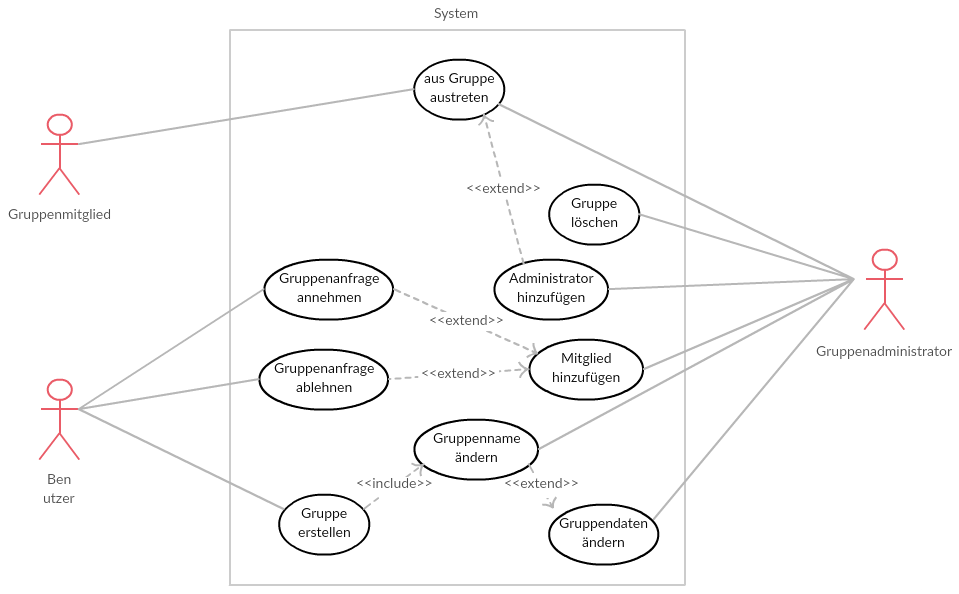
\includegraphics[width=1\textwidth]{Use_Cases/use_case_Gruppen.png}
	\caption{Use-Case Diagramm für Gruppenfunktionen}
\end{figure}



\subsubsection{öffentliche Funktionen}
Die im Folgenden beschriebenen Funktionen sind öffentlich, das bedeutet sie können von jedem Benutzer ausgeführt werden.
Im folgenden Abschnitt wird angenommen, dass der Benutzer ein Benutzerkonto besitzt und bereits im System eingeloggt ist.

\begin{enumerate}[label={\textbf{/F\protect\threedigits{\theenumi}0/}}, leftmargin=*, resume]
%keie Kontakte, sondern Leute direkt über den Benutzernamen in eine Gruppe hinzufügen
	\item \textit{Gruppen anzeigen} \\ %zählt hier "alle gruppen in denen man ist ansehen" als Funktion?
	Ein Benutzer kann sich alle Gruppen, in denen er zu diesem Zeitpunkt Mitglied ist, anzeigen lassen, indem er den 'Gruppen'-Reiter der \gls{Hauptansicht} auswählt (vgl. *GUI-Ansicht*).
	
	\item \textit{Gruppeninformationen abrufen} \label{Gruppeninfo anzeigen} \\%Mitglieder, Admin, aktuelle GOs
	Ein Benutzer, der Mitglied einer Gruppe ist, kann sich von der App Systeminformationen zu dieser Gruppe anzeigen lassen. Dazu wählt der Benutzer das Gruppenicon der gewünschten Gruppe in der *GUI-Ansicht* aus. Darauffolgend werden dem Benutzer vom System folgende Informationen über die Gruppe angezeigt:
	\begin{itemize}
		\item Gruppenname
		\item \colorbox{shadecolor}{Gruppenbild}
		\item \colorbox{shadecolor}{Gruppenbeschreibung}
		\item aktuelle Mitglieder der Gruppe (offene Gruppenmitgliedsanfragen werden nur den Administratoren der Gruppe angezeigt, ehemalige Mitglieder der Gruppe werden nicht angezeigt)
		\item aktuelle Administratoren der Gruppe
		\item aktuelle \glspl{GO} der Gruppe %kann geklickt werden, um in die Ansicht des jeweiligen GOs zu gelangen --> Querverweis einfügen
	\end{itemize}
	
	\item \textit{Gruppe erstellen}\\
	Ein User kann eine neue Gruppe erstellen. Dazu muss in der Ansicht *GUI-Ansicht* die Auswahl "Gruppe erstellen" gewählt werden und anschließend ein Gruppenname angegeben werden. Der Ersteller der Gruppe wird automatisch zum (zu diesem Zeitpunkt) einzigen Gruppenmitglied und Administrator derselben. Um anschließend Mitglieder zu der Gruppe hinzuzufügen, muss die Funktion \ref{Mitglieder hinzufügen} aufgerufen werden.
	
	
	\item \textit{Aus Gruppe austreten}\\
	Ein \gls{Benutzer}, der Mitglied einer Gruppe ist, kann aus derselben austreten. Sollte der Benutzer einziger Administrator der Gruppe sein, muss zuerst ein weiteres aktuelles Mitglied der Gruppe zum Administrator ernannt werden, bevor diese Funktion ausgeführt werden kann (siehe Funktion \ref{Admin hinzufügen}). \\
	Um aus einer Gruppe auszutreten wird vom Benutzer in der Gruppensansicht (vgl. *GUI-Ansicht*) die Detailansicht der ausgewählten Gruppe aufgerufen (vgl. *GUI-Ansicht*) und anschlie"send auf den Button 'Gruppe verlassen' geklickt. Das System entfernt den Benutzer aus der Gruppe und die Funktion ist erfolgreich abgeschlossen. Die Gruppe bleibt im System für alle anderen Benutzer weiterhin bestehen.\\
	In dem Fall, dass der austretende Benutzer das einzige Mitglied der Gruppe ist (und somit auch Administrator), entfällt das Ernennen eines neuen Administrators vor dem Austritt und die Gruppe wird nach dem Ausführen dieser Funktion automatisch vom System gelöscht.
	
	\item \textit{Gruppenanfrage beantworten} \label{Gruppenanfrage beantworten} \\
	Diese Funktion setzt voraus, dass ein Benutzer eine Anfrage auf Gruppenmitgliedschaft von einem anderen Benutzer bekommen hat (vgl. Funktion \ref{Mitglieder hinzufügen}). Dem Benutzer werden offene Gruppenanfragen durch ein grün hinterlegtes Gruppenicon in der Gruppenansicht angezeigt (vgl *GUI-Ansicht*). Durch Klicken auf das Icon wird die Funktion "Gruppenanfrage beantworten" gestartet (vgl. *GUI-Ansicht*). Der Benutzer hat zwei Möglichkeiten auf die Anfrage zu reagieren:
	\begin{itemize}
		\item \textit{Bestätigen} bestätigt der Benutzer die Anfrage, so wird er vom System der Gruppe hinzugefügt. Sie erscheint ab sofort in seiner Gruppenübersicht und der Benutzer hat die Befugnis sämtliche öffentlichen Gruppenfunktionen für die Gruppe aufzurufen.
		\item \textit{Ablehnen} lehnt der Benutzer die Anfrage ab, wird keine weitere Aktion des Systems ausgeführt.
	\end{itemize}
Nach Beantwortung der Anfrage wird diese vom System gelöscht.
\end{enumerate}

\subsubsection{Administratorfunktionen}
Im Folgenden wird angenommen, dass der Benutzer in seinem Benutzerkonto angemeldet und der Administrator einer Gruppe ist.\\
Um eine der folgenden Funktionen ausführen zu können muss der Administrator zunächst in die Gruppeninformationsansicht wechseln (vgl. *GUI-Ansicht* und \ref{Gruppeninfo anzeigen}). Unter der Voraussetzung, dass es sich bei dem Benutzer um einen Administrator dieser Gruppe handelt, wird ihm eine Schaltfläche 'Gruppe bearbeiten' angezeigt. Die Betätigung dieser Schaltfläche startet eine Aktivität, die es dem Benutzer erlaubt Änderungen an der aktuellen Konfiguration der Gruppe vorzunehmen. Es wird im Folgenden Abschnitt angenommen, dass der Benutzer diese Aktivität bereits gestartet hat.

\begin{enumerate}[label={\textbf{/F\protect\threedigits{\theenumi}0/}}, leftmargin=*, resume]

	\item \textit{Gruppendaten "andern}\\
	Ein Administrator kann folgende Daten einer Gruppe ändern:
	\begin{itemize}
	\item Gruppenname
	\item \colorbox{shadecolor}{Gruppenbeschreibung}
	\item \colorbox{shadecolor}{Gruppenbild}
	\end{itemize}
	Dazu gibt er die Änderungen in dem jeweiligen Feld der Änderungsansicht ein und betätigt anschließend den Button 'Änderungen speichern'.
	
	\item \textit{Gruppenmitglied hinzuf"ugen} \label{Mitglieder hinzufügen} \\
	Ein Administrator kann einer Gruppe neue Mitglieder hinzufügen. Dazu wählt er den Button 'Mitglied hinzufügen' aus. Anschließend kann anhand der E-Mailadresse, die beim Login benutzt wurde, nach dem gewünschten Benutzer gesucht werden. Das System zeigt dem Administrator Benutzer an, deren E-Mailadresse der Gesuchten entsprechen. Der Administrator wählt den gewünschten Benutzer aus, woraufhin das System diesem Nutzer eine Gruppenanfrage sendet (siehe \ref{Gruppenanfrage beantworten}). Solange die Gruppenanfrage offen ist, wird das potentielle Gruppenmitglied für die Administratoren der Gruppe angezeigt (Status der Mitgliedschaft ist farblich gekennzeichnet), für normale Gruppenmitglieder sind offene Gruppenanfragen nicht sichtbar.
	
	\item \textit{Gruppenmitglied entfernen}\\
	Ein Administrator kann beliebige Mitglieder der Gruppe entfernen, indem er das rote Minuszeichen neben dem zu entfernenden Benutzer anklickt (vgl. *GUI-Ansicht*) und anschließend die Durchführung der Aktion bestätigt. Der ausgewählte Benutzer wird vom System aus der Gruppe entfernt.
	
	\item \colorbox{shadecolor}{\textit{Admin hinzuf"ugen}} \label{Admin hinzufügen} \\
	Ein Administrator kann ein weiteres Mitglied der Gruppe zum Administrator ernennen. Dazu wählt er den 'Als Admin hinzufügen'-Option neben dem gewünschten Gruppenmitglied aus (vgl. *GUI-Ansicht*). Das System ändert die Rolle des Gruppenmitglieds zu 'Adminsitrator'. Das Gruppenmitglied erhält eine Benachrichtigung (???) über den neuen Status und kann ab sofort alle Funktionen eines Administrators der Gruppe ausführen.
	
	\item \textit{Gruppe l"oschen} \\
	Ein Adminsitrator kann eine Gruppe löschen indem er den "Gruppe löschen"-Button auswählt. Das System löscht die Gruppe. Sie wird ab diesem Zeitpunkt nicht mehr in der Gruppenansicht der Mitglieder angezeigt. Mitglieder erhalten keine Benachrichtigung über die Löschung der Gruppe.
	
\end{enumerate}
	
\subsection{GO-Funktionen}

\subsubsection{Übersicht}
Die GO-Funktionen erlauben das Erstellen, Verwalten und Löschen von sogenannten GOs, also Events bei denen die Standorte der GO-Teilnehmer von System verfolgt und in der App angezeigt werden. Das System unterscheidet zwischen zwei Rollen: Gruppenmitglieder und GO-Verantwortliche. GO-Verantwortliche sind gleichzeitig auch Gruppenmitglieder.

	\begin{figure}[H]
		\centering
		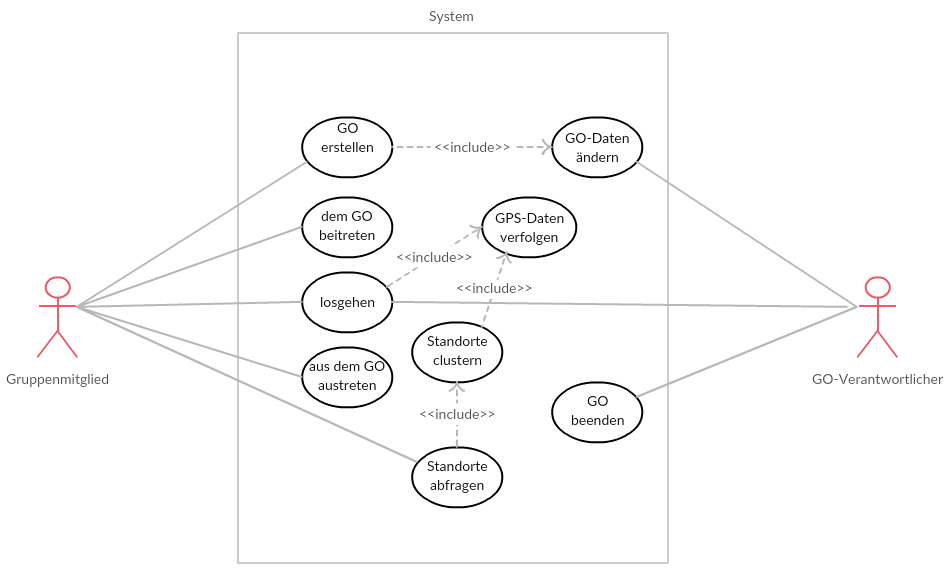
\includegraphics[width=1\textwidth]{Use_Cases/use_case_GO.png}
		\caption{Use-Case Diagramm für GO-Funktionen}
	\end{figure}

 

\subsubsection{öffentliche Funktionen}
Die in diesem Abschnitt beschriebenen Funktionen sind öffentlich, das bedeutet sie können von jedem Benutzer, der Mitglied einer Gruppe ist ausgeführt werden.
Im Folgenden wird angenommen, dass der Benutzer in seinem Benutzerkonto angemeldet und Mitglied einer Gruppe ist.

\begin{enumerate}[label={\textbf{/F\protect\threedigits{\theenumi}0/}}, leftmargin=*, resume]	

	\item \textit{GOs anzeigen}\label{GOs anzeigen} Ein Benutzer kann sich vom System eine Liste seiner aktuellen GOs anzeigen lassen. Dies kann auf zwei verschiedene Arten geschehen:
	\begin{itemize}
		\item Der Benutzer wählt die GO-Hauptansicht (vgl. *GUI-Ansicht*) aus. Das System zeigt eine Liste von allen GOs aus allen Gruppen des Benutzers, für die sein Teilnahmestatus 'Bestätigt' oder 'Unterwegs' ist (vgl. \ref{Teilnahmestatus}).
		\item Der Benutzer wählt die Detailansicht einer seiner Gruppe. Hier wird ihm eine Liste aller GOs dieser Gruppe angezeigt, unabhängig von seinem Teilnahmestatus für dieses GO.
	\end{itemize}
	
	\item \textit{GO-Informationen abrufen} \\
	Ein Benutzer dessen Teilnahmestatus 'Bestätigt' oder 'Unterwegs' ist, kann im System gespeicherte Informationen zu einem GO abrufen (vgl. \ref{GO-Daten}), indem er die Detailansicht des GOs, durch Klicken auf das GO-Icon in der GO-Hauptansicht oder der Gruppendetailansicht (vgl. \ref{GOs anzeigen}), anruft.

	\item \textit{GO erstellen} \\
	Jedes Mitglied einer Gruppe kann für diese Gruppe ein GO erstellen. Dazu wählt der Benutzer in der jeweiligen Gruppendetailansicht die Option 'GO erstellen' und übergibt dem System folgende Informationen (vgl. *GUI-Ansicht*):
	\begin{itemize}
		\item GO-Bezeichnung
		\item Beschreibung
		\item Startzeitpunkt
		\item Endzeitpunkt 
		\item Zielpunkt (optional)
		\item \colorbox{shadecolor}{Clustering-Schwellwert (vgl. \ref{Clustering})}
	\end{itemize}
Der Startzeitpunkt darf nicht in der Vergangenheit liegen.\\
Hat der Benutzer die Angaben bestätigt, wird vom System ein neues GO erstellt und in den Mitgliedern der Gruppe in der Gruppendetailansicht angezeigt. Der Teilnahmestatus aller Gruppenmitglieder wird standardmäßig auf 'Abgelehnt' gesetzt. Der Teilnahmestatus des GO-Verantwortlichen wird auf 'Bestätigt' gesetzt.
Das GO wird den Mitgliedern der Gruppe in der Gruppendetailansicht angezeigt.
Der Ersteller des GOs ist während dem gesamten GO-Lifecycle der GO-Verantwortliche.
	
	\item \textit{Teilnahmestatus ändern}\label{Teilnahmestatus} \\
	Das System weist für jedes GO jedem Gruppenmitglied einen Teilnahmestatus zu. Dieser lautet entweder
	\begin{itemize}
		\item Abgelehnt: Der Benutzer nimmt an dem GO nicht teil
		\item Bestätigt: Der Benutzer nimmt an dem GO teil
		\item Unterwegs: Der Benutzer nimmt an dem GO teil und ist bereits losgegangen
	\end{itemize}
Durch folgende Funktionen kann ein Benutzer seinen Teilnahmestatus in einem GO ändern.

	\begin{itemize}
	\item \textit{Dem Event beitreten} \label{GO-Anfrage} \\
	Mitglieder einer Gruppe können zu jeder Zeit einem aktuellen GO der Gruppe beitreten. Dazu wird vorausgesetzt, dass der aktuelle Teilnahmestatus des Gruppenmitglieds 'Abgelehnt' ist. In der Gruppendetailansicht kann der Benutzer die Option 'Beitreten' des gewünschten GOs anklicken. Das System wird  veranlasst, den Teilnahmestatus des Benutzers auf 'Bestätigt' zu setzen. Sobald dies geschehen ist, kann der Benutzer die GO-Detailansicht (vgl. *GUI-Ansicht*) aufrufen.
	
	\item \textit{Losgehen} \\
	Um diese Funktion ausführen zu können, muss der Teilnahmestatus des Benutzers auf 'Bestätigt' gesetzt sein. Sobald der Button 'Losgehen' betätigt wurde wird der Teilnahmestatus des Benutzers vom System auf 'Unterwegs' gesetzt und die GPS-Verfolgung des Benutzers wird aktiviert und für andere GO-Mitglieder, deren Teilnahmestatus 'Bestätigt' oder 'Unterwegs' ist, sichtbar. Sobald der Startzeitpunkt eintritt, wird der Teilnahmestatus von Benutzern, die 'Bestätigt', aber noch nicht 'Unterwegs' sind, automatisch auf 'Unterwegs' gesetzt.
	
	\item \textit{Aus Event austreten} \\
Ein Benutzer, dessen Teilnahmestatus des GOs 'Bestätigt' oder 'Unterwegs' ist, kann seinen Status auf 'Abgelehnt' setzen, indem er in der GO-Detailansicht den Button 'Aus Event austreten' klickt. Das System setzt den Teilnahmestatus des Benutzers auf 'Abgelehnt. Sollte die GPS-Verfolgung dieses GOs bereits aktiviert worden sein, wird sie vom System deaktiviert. Das System lädt die GO-Hauptansicht des Benutzers.
	
	\item \textit{Anhalten} \\
	Ein Benutzer dessen Teilnahmestatus 'Unterwegs' lautet kann diesen zurück auf 'Bestätigt' setzen, indem er die Option 'Anhalten' auswählt. Das System ändert den Teilnahmestatus und stoppt die GPS-Verfolgung des Benutzers.
	
	\end{itemize}
	
	Bemerkung: Ein GO-Verantwortlicher kann nicht aus dem GO austreten. Der Teilnahmestatus eines GO-Verantwortlichen kann nur 'Bestätigt' oder 'Unterwegs' lauten.\\
	
	\begin{figure}[H]
		\centering
			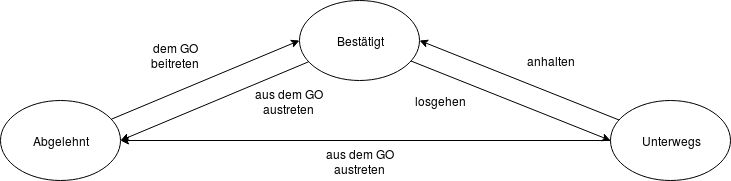
\includegraphics[scale=0.55]{res/Teilnahmestatus.png}
		\caption{Übergangsdiagramm für GO-Teilnehmerstatus}	
	\end{figure}
	
	
	\item \textit{Standorte abfragen}\label{Standorte abrufen} \\
	Ein Benutzer dessen Teilnahmestatus 'Bestätigt' oder 'Unterwegs' ist, kann, bei gestarteten GOs, die Standorte der Gruppenmitglieder abrufen, deren Teilnahmestatus 'Unterwegs' ist. Dazu ruft er die GO-Detailansicht auf'. Das System zeigt auf einer Karte die anonymisierten und ggf. zu Clustern zusammengefassten Standorte der losgegangen Benutzer an (vgl. \ref{Clustering}).
	
\end{enumerate}

\subsubsection{Funktionen für GO-Verantwortliche}
Im Folgenden wird angenommen, dass der Benutzer in seinem Benutzerkonto angemeldet ist und der Verantwortlicher eines GOs ist.

\begin{enumerate}[label={\textbf{/F\protect\threedigits{\theenumi}0/}}, leftmargin=*, resume]	
	\item \textit{GO-Daten ändern} \\
	Der GO-Verantwortliche kann auch nach Erstellung des GOs die/den
	\begin{itemize}
		\item GO-Bezeichnung
		\item Startzeitpunkt
		\item Endzeitpunkt
		\item Zielpunkt
		\item \colorbox{shadecolor}{Clustering-Schwellwert (vgl. \ref{Clustering})}
	\end{itemize}
	ändern. Der neue Startzeitpunkt darf nicht in der Vergangenheit liegen. Sobald die Änderungen vom Benutzer bestätigt wurden, werden sie vom System übernommen und den Mitgliedern des GOs angezeigt, wenn diese die GO-Detailansicht aufrufen. Die GO-Daten können nicht mehr geändert werden, sobald der Startzeitpunkt eingetreten ist.
	
	\item \textit{GO beenden} \\
	Ein GO kann vom GO-Verantwortlichen vorzeitig beendet werden durch Klicken des Buttons 'GO beenden' in der GO-Detailansicht. Das System registriert das GO als beendet und sendet eine Benachrichtigung an alle Gruppenmitglieder mit Teilnahmestatus 'Bestätigt' und 'Unterwegs'. Anschließend wird das GO vom System gelöscht. \\
	Wird das GO nicht vom GO-Veratnwortlichen vorzeitig beendet, wird es bei Erreichen des Endzeitpunkts automatisch vom System beendet. Das System führt dabei die gleichen Aktionen aus wie beim Beenden durch den GO-Verantwortlichen.
	
	\item \textit{GO löschen} \\
	Ein Go kann von dem GO-Verantwortlichen gelöscht werden. Dazu gibt es in der GO-Datailansicht den Button 'GO löschen'. Ein GO kann jederzeit gelöscht werden.
\end{enumerate}

\subsubsection{Systemfunktionen}
Die im folgenden beschriebenen Funktionen werden vom System ausgeführt, ohne das die Ausführung von einer direkten Interaktion mit dem Benutzer ausgelöst muss.
\begin{enumerate}[label={\textbf{/F\protect\threedigits{\theenumi}0/}}, leftmargin=*, resume]	
	%\item \textit{Verwaltung von Server Log-Dateien}
	
	\item \textit{Standorte verfolgen}\\
	Das System verfolgt die Standorte aller Benutzer, dessen Teilnahmestatus für das GO auf 'Unterwegs' gesetzt ist. Die Standortverfolgung ist so lange aktiviert, bis sich der Teilnahmestatus des Benutzers ändert oder das GO beendet wird. Sie wird auch weiter durchgeführt, sollte der Benutzer die App nur im Hintergrund ausführen.
	
	\item \textit{Clustering}\label{Clustering} \\
	Ist der Teilnahmestatus eines Benutzers in einem aktiven GO auf 'Unterwegs' gesetzt, beginnt das System den Standort dieses Benutzers zu erfassen. Die Standorte der losgegangenen Benutzer werden gegebenenfalls geclustert, sodass in der App nicht der Standort der einzelnen Benutzer, sondern die gemittelte Position dieser Benutzer angezeigt wird. Die Positionen mehrerer Benutzer werden zu einem Cluster zusammengefasst, sobald die Distanz der einzelnen Personen zum Zentrum des Clusters einen kritischen Schwellwert unterschreitet. \\ 
	
	\colorbox{shadecolor}{\parbox{.9\textwidth}{Dieser Schwellwert kann in den GO-Daten vom GO-Verantwortlichen bestimmt werden.}}\\
	
	 Es werden dem Benutzer beim Abrufen der Standorte (\ref{Standorte abrufen}) in einem GO die errechneten Standortcluster der anderen Benutzer angezeigt und wie viele Benutzer sich jeweils in einem Cluster befinden. Die Standorte von Benutzern, die sich nicht in der Nähe von anderen Benutzern befinden, werden nicht-geclustert dargestellt.
	
\item \textit{Anonymisierung der Benutzer}\label{Anonymisierung} \\ Die Funktionalität des Systems soll die Anonymität des Benutzers bestmöglich sicherstellen. Dazu sind folgende Funktionen der App zu implementieren:
		\begin{itemize}
			\item Die Standorte der Benutzer während eines GOs werden auf der Karte ohne den jeweiligen Benutzernamen angezeigt und bei ausreichender geographischer Nähe nur in Clustern dargestellt
			\item \colorbox{shadecolor}{\parbox{0.85\textwidth}{Die Genauigkeit der Standortbestimmung kann durch den Clustering-Schwellwert von dem GO-Verantwortlichen selbst bestimmt werden.}}
			\item \colorbox{shadecolor}{\parbox{.85\textwidth}{Bei GOs, bei denen weniger als 5 Benutzer die Standortverfolgung aktiviert haben, erhält der Benutzer beim Losgehen eine Warnung: er kann den Start der Standortverfolgung solange verzögern, bis mindestens 4 andere Benutzer ebenfalls losgegangen sind.}}
			\item Der automatische Start der Standortverfolgung bei Eintreten des Startzeitpunkts wird im Fall von weniger 5 losgegangen Benutzern nicht ausgeführt. Die Benutzer müssen manuell die Standortverfolgung durch Änderung des Teilnahmestatus auf 'Unterwegs' aktivieren.
			\item Benutzer haben zu jeder Zeit die Möglichkeit die Standortverfolgung zu beenden, indem sie ihren Teilnahmestatus auf 'Abgelehnt' oder 'Bestätigt' setzen.
		\end{itemize}
		Bemerkung: In Ausnahmefällen kann die Anonymität eines Benutzers nicht garantiert werden (etwa, wenn er sich als einziger nicht in der Nähe der anderen GO-Teilnehmer befindet oder das GO nur sehr wenige Teilnehmer hat). Das System weist den Benutzer bei erstmaliger Anmeldung auf diese Tatsache hin. Der Benutzer muss sich damit einverstanden erklären, bevor er die App nutzen kann (vgl. \ref{Registrieren}).
		
\end{enumerate}

\subsection{Sonstiges}
Im Folgenden wird angenommen, dass der Benutzer in seinem Benutzerkonto angemeldet ist.

\begin{enumerate}[label={\textbf{/F\protect\threedigits{\theenumi}0/}}, leftmargin=*, resume]	
 \item \colorbox{shadecolor}{\textit{Benachrichtigungen senden}}\\
	Die App sendet dem Benutzer Android-Benachrichtigungen bei folgenden Ereignissen:
	\begin{itemize}
		\item Der Benutzer wurde zu einer Gruppe hinzugefügt
		\item In einer Gruppe des Benutzers wurde ein GO erstellt
		\item ein GO des Benutzers ist gestartet
	\end{itemize}
	\item \colorbox{shadecolor}{\textit{Benachrichtigungseinstellungen ändern}} \\
	Der Benutzer kann entscheiden, ob er Android-Benachrichtigungen von der App erhalten will oder nicht. Er kann dies selbst über einen Slider in der Einstellungs-Ansicht einstellen (vgl. *GUI-Ansicht*). Die default-Einstellung ist 'stumm', d.h. der Benutzer erhält keine Benachrichtigungen der App auf seinem Android-Gerät.
	\item \textit{About-Seite anzeigen} \\
	Der Benutzer kann eine 'About'-Seite aufrufen, die allgemeine Informationen zur App beinhaltet.
	\item \textit{Lizenzinformationen anzeigen} \\
	Der Benutzer kann Informationen zur Lizenz der App einsehen.
\end{enumerate}

\newpage
\section{Produktdaten}

\begin{enumerate}[label={\textbf{/D\protect\threedigits{\theenumi}0/}}, leftmargin=*]
	\item \textit{Profildaten} \label{Profildaten} Für jeden im System registrierten Benutzer m"ussen folgende Informationen gespeichert werden:
		\begin{itemize}
			\item \textit{Benutzerkennung}
				\begin{itemize}
					\item Benutzer-ID (eindeutig, erzeugt von der verwendeten Firebase Authentication)
					\item E-Mailadresse des zum Anmelden verwendeten Google-Accounts
				\end{itemize}
			\item \textit{Persönliche Daten} \label{persönliche Daten} 
			\begin{itemize}
			\item Benutzername (defaultwert: E-Mailadresse des Benutzers)
			\item Profilbild
			\item Gruppen
		\end{itemize}
		\end{itemize}
	
	\item \textit{Gruppendaten} Für jede erstellte Gruppe müssen folgende Informationen gespeichert werden:
	\begin{itemize}
		\item Gruppen-ID (eindeutig)
		\item Gruppenname
		\item Gruppenbild
		\item Gruppenbeschreibung
		\item Mitglieder
		\item Administratoren
		\item offene Gruppenanfragen %--> wie sollte man länger ausstehende Anfragen verwalten?
		\item aktuelle GOs
	\end{itemize}
	\item \textit{GO-Daten} \label{GO-Daten}
	Für jedes erstellte GO müssen folgende Informationen gespeichert werden:
	\begin{itemize}
		\item GO-ID (eindeutig)
		\item GO-Verantwortlicher
		\item Startzeitpunkt
		\item Endzeitpunkt
		\item Zielort (optional)
		\item Clustering-Schwellwert
		\item Gruppe, der das GO angehört
		\item Gruppenmitglieder mit Teilnahmestatus 'Abgelehnt'
		\item Gruppenmitglieder mit Teilnahmestatus 'Bestätigt'
		\item Gruppenmitglieder mit Teilnahmestatus 'Losgegangen'
		\item Standorte der losgegangenen Benutzer
	\end{itemize}
\end{enumerate}

\newpage
\section{Nichtfunktionale Anforderungen}
\begin{enumerate}[label={\textbf{/NF\protect\threedigits{\theenumi}0/}}, leftmargin=*]
		\item \textit{Anonymisierung des Standortes} \\
		Um den Datenschutz, beziehungsweise die Privatsphäre der Benutzer zu garantieren, findet die Lokalisierung und Mittlung der Standorte(via GPS) der Mitglieder einer Gruppe, die sich einem Event angeschlossen haben, erst ab einer Teilnehmerzahl von 3 statt. 
		
		\item \textit{Eventlimit} \\
		Die Anzahl an gleichzeitig möglichen Events ist auf 10 beschränkt um mögliche Überlastungen des Servers durch Schadsoftware oder böswillige Nutzer zu verhindern.
		
		\item \textit{Mitgliederanzahl} \\
		Das Limit an maximal zugelassen Mitgliedern wird auf 50 beschränkt um die Füllung von Gruppen mit vielen inaktiven Mitgliedern zu verhindern. Die App ist auf kleine Gruppen und Ansammlungen ausgelegt.
		
		\item \textit{Menüsortierung} \\
		Sowohl Gruppenübersicht als auch die Übersicht der Gruppenmitglieder ist alphabetisch(anhand des Benutzernamens) sortiert. 
		
		\item \textit{Serverlimit} \\
		Der Server erlaubt ein Maximum von 300 möglichen Gruppen und 5000 Nutzern.
		
		\item \textit{Standortaktualisierungszeit} \\
		Die Aktualisierung der Standortmittlung findet alle 8 Sekunden statt.
		
		\item \textit{Automatisches Ausloggen} \\
		Der Nutzer wird nicht automatisch ausgeloggt sollte die App inaktiv oder geschlossen werden. Nur im Falle, dass der Nutzer sich auf einem anderen Gerät einloggt wird er auf dem vorigen ausgeloggt.
		
		\item \textit{Startzeit} \\
		Die Startzeit der App sollte nicht länger als 5 Sekunden betragen.
		
\end{enumerate}

\newpage
\section{Benutzeroberfläche}
%TODO Übergangsdiagramm erstellen

\newpage
\section{Qualitäts-Zielbestimmungen}
Bestimmung der Schwerpunkte in der Entwicklung dieser App:
\begin{enumerate}
	\item[Bedienbarkeit] Eine möglichst einfache Bedienung mit voller Funktionalität.
	\item[Verständnis] Ein simples Design, dass direktes Verständnis der Funktionen und Arbeitsweise der App erlauben.
	\item[Funktionalität] Möglichst intuitive Umsetzung der gewünschten Funktionen der App.
	\item[Modifizierbarkeit] Die einfach Änderung und Erweiterung der Funktionalität der App.
\end{enumerate}
% Funktionalität, Zuverlässigkeit, Benutzbarkeit, Effizienz, Änderbarkeit, Übertragbarkeit

\newpage
\section{globale Testfälle und Testszenarien}

\subsection{Erstellen, Verwalten, Löschen eines Benutzeraccounts}

\subsubsection*{Szenario 1}Bob will die App GO nutzen. Dazu erstellt er einen Benutzeraccount, fügt persönliche Daten seinem Benutzerprofil hinzu und loggt sich anschließend wieder aus.\\

\textbf{Akteure:} Bob (Benutzer) \\

\textbf{Voraussetzungen: }Bob benutzt ein Smartphone, dass sämtliche Betriebsbedingungen erfüllt (vgl. \ref{Betriebsbedingungen}) erfüllt und auf dem die App installiert ist. Bob verfügt über ein gültiges Google-Konto.\\

\textbf{Testfälle:}
\begin{enumerate}[label={\textbf{/T\protect\threedigits{\theenumi}0/}}, leftmargin=*]
	\item\label{Registrieren-Test} Bob öffnet die App, gibt die Anmeldedaten seines Google-Accounts ein und klickt auf den Button 'Sign In'.
	\item Bob ist in seinem Benutzeraccount angemeldet. Bob öffnet seine Profilansicht und klickt auf den Button 'Profil ändern'. Er gibt in das Textfeld 'Benutzername' den Namen 'Bob' ein. Er klickt auf den Button 'Bild wählen'. Er wählt ein Bild aus dem Foto-Ordner des Android-Geräts aus. Er klickt auf den Button 'Änderungen speichern'.
	\item Bob ist in seinem Benutzeraccount angemeldet. Bob öffnet die Ansicht 'Einstellungen' und klickt auf das Feld 'Abmelden'.
\end{enumerate}

\subsubsection*{Szenario 2}Bob will die App GO nicht mehr benutzen. Er will deshalb seinen Benutzeraccount löschen. \\

\textbf{Akteure:} Bob (Benutzer) \\

\textbf{Voraussetzungen: }Bob besitzt einen gültigen GO-Benutzeraccount.\\

\textbf{Testfälle:}
\begin{enumerate}[label={\textbf{/T\protect\threedigits{\theenumi}0/}}, leftmargin=*, resume]
	\item Bob meldet sich in seinem Benutzeraccount an. 
	\item Bob ist in seinem Benutzeraccount angemeldet. Er öffnet seine Profilansicht und klickt auf den Button 'Profil löschen'.
\end{enumerate}

\subsection{Erstellen, Verwalten, Löschen einer Gruppe}

\subsubsection*{Szenario 3} Bob, Alice und Peter wollen gemeinsam eine Gruppe erstellen, um ihre Treffen organisieren zu können. Bob soll der Administrator dieser Gruppe sein.\\

\textbf{Akteure:} Bob (Administrator), Alice (Gruppenmitglied), Peter (Gruppenmitglied) \\

\textbf{Voraussetzungen: }Bob, Alice und verfügen beide über einen gültigen GO-Benutzeraccount.

\textbf{Testfälle:}
\begin{enumerate}[label={\textbf{/T\protect\threedigits{\theenumi}0/}}, leftmargin=*, resume]
	\item Bob klickt in der Gruppenansicht auf das Feld 'neue Gruppe'. Er gibt in das Eingabefeld den Gruppennamen 'Foo' ein.
	\item Bob öffnet die Gruppendetailansicht und klickt auf den Button 'Gruppe bearbeiten'. Er gibt den Gruppennamen 'Bar' und die Gruppenbeschreibung 'FooBar' ein.
	\item Bob öffnet die Gruppenansicht der App. Ihm wird die gruppe 'Bar' angezeigt.
	\item Bob öffnet die Gruppendetailansicht und klickt auf das Feld 'Mitglied hinzufügen'. Er gibt in das Suchfeld Alice's E-Mailadresse ein. Er wählt aus den Suchresultaten Alice's Profil aus. Er wiederholt den Vorgang, um Peter ur Gruppe hinzuzufügen.
	\item Alice hat eine Gruppenanfrage für die Gruppe 'Bar' bekommen. Sie bestätigt die Gruppenanfrage.
	\item Peter hat eine Gruppenanfrage für die Gruppe 'Bar' bekommen. Er lehnt die Gruppenanfrage ab.
	\item Alice ruft die Gruppendetailansicht auf. Ihr werden folgende Informationen angezeigt:
	\begin{itemize}
		\item Gruppenname: Bar
		\item Gruppenbeschreibung: FooBar
		\item Mitglieder: Bob, Alice
		\item Administratoren: Bob
		\item aktuelle GOs: leer
	\end{itemize}
\end{enumerate}

\subsubsection*{Szenario 4}Nach dem Event wollen Bob, Alice und Peter die Gruppe 'Bar' wieder auflösen.\\

\textbf{Voraussetzungen: }Bob, Alice und Peter verfügen über je einen gültigen GO-Benutzeraccount. Bob, Alice und sind gemeinsam Mitglieder der Gruppe 'Bar'. Bob ist Administrator, Alice und Peter sind Gruppenmitglieder.

\textbf{Akteure:} Bob (Administrator), Alice (Gruppenmitglied), Peter (Gruppenmitglieder) \\

\textbf{Testfälle:}
\begin{enumerate}[label={\textbf{/T\protect\threedigits{\theenumi}0/}}, leftmargin=*, resume]
	\item Bob wählt in der Gruppendetailansicht der Gruppe 'Bar' die Option 'Austreten'. Die Aktion schlägt fehl, da Bob der einzige Administrator der Gruppe ist.
	\item Bob wählt in der Gruppendetailansicht der Gruppe 'Bar' die Option 'Administrator hinzufügen'. Er wählt Alice als neuen Administrator aus.
	\item Bob wählt in der Gruppendetailansicht der Gruppe 'Bar' die Option 'Austreten'. Die Aktion ist erfolgreich.
	\item Alice entfernt Peter aus der Gruppe 'Bar'
	\item Alice wählt in der Gruppendetailansicht die Option 'Gruppe löschen'.
\end{enumerate}

\subsection{Erstellen, Verwalten und Löschen eines GOs}

\subsubsection*{Szenario 5}Bob erstellt ein neues GO in der Gruppe 'Bar'. Alice tritt dem GO bei und bestätigt 10min vor dem Startzeitpunkt, dass sie losgegangen ist.\\

\textbf{Akteure:} Bob (GO-Verantwortlicher), Alice (Gruppenmitglied)\\

\textbf{Voraussetzungen: }Bob und Alice sind Mitglieder der Gruppe 'Bar'. Die Gruppe hat eine Gesamtmitgliederzahl von 5 Benutzern.

\textbf{Testfälle:}
\begin{enumerate}[label={\textbf{/T\protect\threedigits{\theenumi}0/}}, leftmargin=*, resume]
	\item\label{Go Test} Bob erstellt ein GO mit folgenden Daten:
	\begin{itemize}
		\item Startzeitpunkt: 15.09.17 14:00
		\item Endzeitpunkt: 15.09.2017 16:00
		\item Zielort: leer
		\item Clustering-Schwellwert: 100m
	\end{itemize}
	\item Alice ruft die Go-Datailansicht auf, um sich über das GO zu informieren. Ihr werden die Informationen aus Testfall \ref{Go Test} angezeigt.
		\item Alice setzt ihren Teilnahmestatus auf 'Bestätigt'.
	\item Alice setzt ihren Teilnahmestatus manuell auf 'Unterwegs'.
	\item zum Startzeitpunkt setzt das System Bobs Teilnahemstatus automatisch auf 'Unterwegs' (es ist vorausgesetzt, dass alle anderen Gruppenmitglieder bereits losgegangen sind).
	\item alle Gruppenmitglieder außer Bob sind als Gruppe (geographisch nah beieinander) unterwegs. Bob kann die Standorte der anderen Gruppenmitglieder nur als Cluster auf der Karte sehen.
	\item (a) das GO wird von Bob manuell beendet. \\
	 (b) das GO endet zum Endzeitpunkt automatisch.	
\end{enumerate}

\subsubsection*{Szenario 6} Die Pläne der Gruppe ändern sich. Bob muss die Details des GOs ändern. Letztendlich muss das Treffen komplett abgesagt werden, also wird das GO von Bob gelöscht.\\

\textbf{Akteure:} Bob (GO-Verantwortlicher)\\

\textbf{Voraussetzungen: }Bob hat zuvor ein GO erstellt mit den GO-Daten aus Testfall \ref{Go Test} und ist der GO-Verantwortliche. Das Go hat noch nicht begonnen.\\

\textbf{Testfälle:}\\
\begin{enumerate}[label={\textbf{/T\protect\threedigits{\theenumi}0/}}, leftmargin=*, resume]
	\item Bob ruft die GO-Detailansicht auf und ändert den Startzeitpunkt des GOs von 15.09.17 14:00 auf 18.09.17 15:00
	\item Bob löscht das GO
\end{enumerate}

\subsubsection*{Szenario 7}Alice entfernt sich während des GOs von der Gruppe. Sie will nicht, dass man ihren Standort verfolgen kann, deshalb setzt sie ihren Teilnahmestatus von 'Unterwegs' auf 'Bestätigt'. Nach einer Weile entschließt sie sich nicht mehr zu der Gruppe zurückzukehren und verlässt das GO.\\

\textbf{Akteure:} Bob (GO-Verantwortlicher), Alice (Gruppenmitglied)\\

\textbf{Voraussetzungen: }Alice ist Mitglied einer Gruppe. Es findet aktuell ein GO statt. Alice's Teilnahmestatus für dieses GO lautet 'Unterwegs'.\\

\textbf{Testfälle:}
\begin{enumerate}[label={\textbf{/T\protect\threedigits{\theenumi}0/}}, leftmargin=*, resume]
	\item Alice ändert ihren Teilnahmestatus auf 'Bestätigt
	\item Alice ändert ihren Teilnahmestatus auf 'Abgelehnt'
\end{enumerate}

\subsection{Sonstiges}

\subsubsection*{Szenario 8} Bob will sich über die App GO informieren und schaut sich dazu die About- und Lizenzinformnationsseiten der App an.\\

\textbf{Akteure: }Bob (Benutzer)\\

\textbf{Voraussetzungen: }Bob Bob besitzt einen gültigen GO-Benutzeraccount.\\

\textbf{Testfälle:}\\
\begin{enumerate}[label={\textbf{/T\protect\threedigits{\theenumi}0/}}, leftmargin=*, resume]
	\item Bob ruft die About-Seite der App auf.
	\item Bob ruft die Lizenzinformationen der App auf.
\end{enumerate}

\subsubsection*{Szenario 9} Bob und Alice erstellen gemeinsam eine neue Gruppe mit Alice als Administrator. Bob aktiviert die Benachrichtigungen der App, um zeitnah mitzubekommen, wenn es Neuigkeiten in der Gruppe gibt.\\

\textbf{Akteure: }Bob (Gruppenmitglied), Alice (Administrator)\\

\textbf{Voraussetzungen: }Bob und Alice besitzen beide einen gültigen GO-Benutzeraccount. Alice ist Administrator der Gruppe 'Foo'.\\

\textbf{Testfälle:}\\
\begin{enumerate}[label={\textbf{/T\protect\threedigits{\theenumi}0/}}, leftmargin=*, resume]
	\item Bob ändert die Benachrichtigungseinstellungen in seinem Profil auf 'aktiv'.
	\item Alice fügt Bob der gruppe 'Foo' hinzu. Bob bekommt eine Benachrichtigung auf seinem Android-Gerät.
	\item Alice erstellt einen neuen GO in der Gruppe 'Foo'. Bob bekommt eine Benachrichtigung auf seinem Android-Gerät.
	\item Der Startzeitpunkt des GOs ist eingetreten. Bob bekommt eine Benachrichtigung auf seinem Android-Gerät.
\end{enumerate}

\newpage
\section{Anhang}

\newpage
\printglossary	
\end{document}



\grid
